\documentclass[12pt,a4paper]{article}
\usepackage[latin2]{inputenc}
\usepackage{graphicx}
\usepackage{ulem}
\usepackage{amsmath}
\begin{document}
docx2tex

Kriszti�n P�cza, Mih�ly Bicz�, Zolt�n Porkol�b

E�tv�s Lor�nd University, Faculty of Informatics, Department of 
Programming Languages and Compilers, P�zm�ny P�ter s�t�ny 1/C. H-1117, 
Budapest, Hungary 

kpocza@kpocza.net, mihaly.biczo@t-online.hu, gsd@elte.hu 

\textbf{Abstract}

Docx2tex is a small command line tool that uses standard technologies to 
help users of Word 2007 to publish publications where typography is 
relevant or only papers produced by TeX are accepted. Behind the scenes, 
docx2tex uses common technologies to interpret Word 2007 OOXML format 
without utilizing the API of Word 2007. Docx2tex is planned to be 
published as a free open source utility that is accessible and 
extensible by everyone. This paper has been originally written in Word 
2007 and then converted to TeX using docx2tex.

\section{Introduction}
There are two general methods to produce human readable and printable 
digital documents:

\newcounter{numberedCntA}
\begin{enumerate}
\item Using a WYSIWYG word processor
\item Using a typesetting system
\setcounter{numberedCntA}{\theenumi}
\end{enumerate}
Each of them has its own advantages and disadvantages therefore each of 
them has many use cases where one is better than the other and vice 
versa.

WYSIWYG $[$1$]$ is the acronym for the term \textit{What You See Is 
What You Get} that originates from the late '70. WYSIWYG editors are 
mostly used by everyday computer users whose aim is to produce good 
looking documents fast and exploit the rich formatting capabilities of 
such systems. WYSIWYG editors and word processors ensure that the 
printed version of the document will be the same as the document that is 
visible on the screen during editing. The first WYSIWYG word processor 
called Bravo was created at Xerox by Charles Simonyi, who was the 
inventor of intentional programming. In 1981 Simonyi left Xerox and 
joined Microsoft where he created Microsoft Word $[$2, 3$]$, the first 
and to this day the most popular word processor. Word is capable to 
produce simple and also complex documents even with a lot of 
mathematical symbols. The other important feature of Word is \textit{
Track Changes} that supports team work where any of the team members 
can modify the document while these modifications are tracked and can be 
accepted or refused by the team leader.

Typesetting is the process of putting characters of different type to 
their correct place on the paper or screen. Before electronic 
typesetting systems became widely used, printed materials had been 
produced by compositors who worked by hand or by special machines. The 
aim of typesetting systems is to create high quality output of materials 
that may contain complex mathematical formulae and complex figures. 
Similarly, electronic typesetting systems follow this goal and produce 
high quality, device independent output. The most popular typesetting 
system is TeX $[$4$]$ created by Donald E. Knuth. TeX is mainly used by 
researchers and by individuals whose aim is to achieve the best quality 
printout and platform or device independence. The users of TeX use a 
special and extensible DSL (Domain Specific Language) that was designed 
to solve complex typesetting problems or even produce books containing 
hundreds of pages.

There is a big gap between these systems because each tries to satisfy 
different demands, which are: produce common documents fast even in 
teamwork vs. achieve the best quality and typographically correct 
printout. To converge them there are some commercial and non-commercial 
tools that support conversion from Word or other WHYSIWYG formats to TeX 
(and back). The first direction, converting from WHYSIWYG (Word) formats 
to TeX, has more reason for existence because many users edit the 
original text in Word for the sake of simplicity and efficiency, and 
later convert it to TeX by hand in order to ensure quality 

The problems with present applications supporting this scenario are the 
following:

\newcounter{numberedCntB}
\begin{enumerate}
\item Many of them are available only as commercial tools
\item They have limitations (running times or page limit) when not 
purchased 
\item Support only the old, binary Word or Rich Text document format 
(.doc, .rtf)
\item Use the COM API of Word to process documents that makes them 
complex
\setcounter{numberedCntB}{\theenumi}
\end{enumerate}
In this paper we present an open source and free solution that is 
capable of handling the new and open Word 2007 .docx format natively by 
using standard technologies without leveraging the COM API of Word and 
even without installing Word. In this article the current features are 
presented along with further development directions.

\section{Existing Solutions}
It has been also a big challenge to convert proprietary, binary or 
simply other document formats to TeX. Because Word is the most common 
editor therefore most of the tools convert from Word documents. One of 
these tools is \textit{Word2TeX} $[$5$]$, that makes Word capable to 
save documents in TeX format. This tool is embedded into Word, has an 
evaluation period and can be purchased in different license packages. A 
similarly featured tool called \textit{Word-to-Latex} $[$6$]$ is 
closed source and free software. 

There is a possibility to use OpenOffice.org $[$7$]$ that is capable of 
reading Word documents and also saving them in TeX format. It is a free 
and open source application; however it interprets the binary data of 
Word documents.

Rtf2latex2e $[$8$]$ is the most recent solution that translates .rtf 
files to TeX. It is a free and open source application. 

\section{Technology}
In this section we will enumerate and then shortly review the 
technologies that are used in docx2tex and show how they cooperate.

The used technologies are the following:

\newcounter{numberedCntC}
\begin{enumerate}
\item Office Open XML (ECMA 376 Standard $[$9$]$, recently approved as 
an ISO Standard), the default format of Word 2007. Shortly: OOXML.
\item Microsoft .NET 3.0 (CLI is ECMA 335 Standard $[$10$]$ and ISO/IEC 
23271:2006 Standard $[$11$]$)
\item ImageMagick $[$12$]$ to convert images 
\setcounter{numberedCntC}{\theenumi}
\end{enumerate}
OOXML files are simplistically XML and media files compressed using ZIP. 
Docx2tex uses Microsoft .NET 3.0 to open and unzip OOXML Word 2007 .docx 
documents. Microsoft .NET 3.0 has some special classes in the \textit{
System.IO.Packaging} namespace that facilitate opening and unzipping 
OOXML files and abstract the contained XML and media files as packages. 
The operations performed by this component are described by the object 
line called \textit{OOXML depackaging} in \ref{figure:_Ref194044987}..

The most important component of docx2tex is the \textit{Core XML Engine
} that implements the base foundations of conversation from XML files to 
TeX. The Core Engine is responsible for reading and processing the XML 
data of the OOXML documents that is served by the OOXML depackaging 
component. The Core Engine identifies parts of the OOXML document and 
processes the contents of these parts (paragraphs, runs, tables, image 
references, numberings, \ldots ). It is not responsible for processing 
parts of the OOXML document that are available through a relation. 
Docx2tex has a set of internal \textit{Helper functions} that are 
responsible for driving the processing of related entities like image 
conversion, special styling and resolve the properties of numbered list.

When an image reference is found in the XML, ImageMagick is called to 
produce EPS files from the original image files. The resulting EPS files 
can be simply embedded into TeX documents. 

We support the exact output produced by Word 2007, other outputs saved 
by third party applications that may differ the ECMA 376 Standard are 
not supported.

In the next sections the structure of OOXML will be shortly discussed 
where we will review \textit{runs}. A \textit{run} is a piece of 
text which also has some style specification. Runs are placed and 
removed dynamically while the word document is edited. A sentence or 
even a word can be divided to more than one run with the same style. The 
component called \textit{TeXizer} is responsible to join runs having 
the same style to a simple run in the outgoing TeX code and break the 
lines length at some predefined value (default is 72).

The previous description is illustrated by the following UML sequence 
diagram:

\begin{figure}[h]
\centering
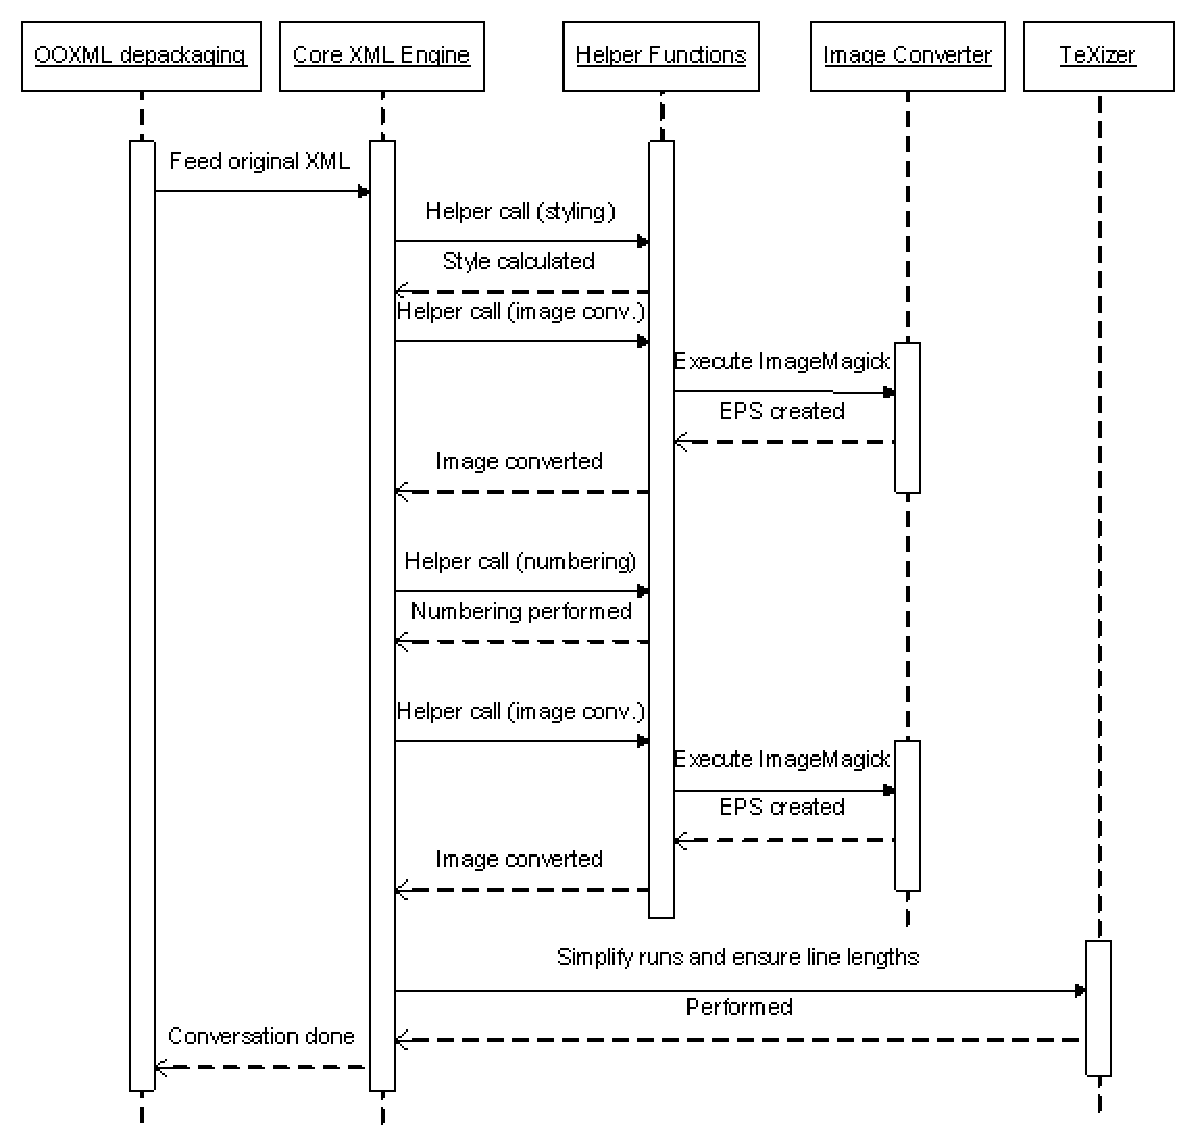
\includegraphics[width=14.20cm,height=13.60cm]{media/image1.eps}
\caption{\label{figure:_Ref194044987}: UML sequence diagram}
\end{figure}



\section{Features of Docx2tex}
In this section we first present the supported and then the unsupported 
features of docx2tex.

\subsection{Supported Features}
Docx2tex supports the following features of Word 2007 and TeX:

\newcounter{numberedCntD}
\begin{enumerate}
\item Normal text
\item Italic, bold, underlined, stroked, small capitals, \ldots 
\item Left, right, center aligned text
\item Headings - sections (3 levels)
\item Verbatim text
\item Style mapping
\item Simple tables
\item Line and page breaks 
\item Numbered and bulleted lists
\item Multilevel lists and continuous numbered lists
\item Figure, table and listing captions
\item Cross reference to captions and headings
\item Image conversion from various formats (incl. .png and .jpeg) to 
.eps
\item Substitution of special characters (e.g. $\backslash$, \#, \{, \}, 
$[$, $]$, \%, \&, \~, \ldots )
\item Text boxes
\setcounter{numberedCntD}{\theenumi}
\end{enumerate}
docx2tex supports normal and special text styles and also text 
alignments. We support heading styles \textit{Heading1}, \textit{
Heading2}, and \textit{Heading3} that convert to \textit{
$\backslash$section}, \textit{$\backslash$subsection}, and \textit{
$\backslash$subsubsection} respectively. Word does not support verbatim 
text while TeX does. To workaround this deficiency, text marked with 
\textit{Verbatim} style is converted to \textit{verbatim} text 
surrounded by \textit{$\backslash$begin\{verbatim\}} and \textit{
$\backslash$end\{verbatim\}}. There are many cases when we are 
required to use different styles for headings or even verbatim. 

Only simple, left aligned tables are supported. Both numbered and 
bulleted lists are supported, moreover these lists can be embedded 
together and continuous lists are also supported using the \textit{
$\backslash$setcounter}, the \textit{$\backslash$enumi}, and the 
\textit{$\backslash$theenumi} commands. Figure, table and listings 
captions are recognized and we support referencing them together with 
heading references also. Image references are resolved and the images 
(mainly .png and .jpeg) embedded in the OOXML documents are converted to 
.eps. The width and height properties are queried and the same 
properties are used in the resulting TeX documents. Some special TeX 
characters are also resolved and escaped in the resulting TeX document. 
Text found in \textit{Text Boxes} of Word documents are also processed 
and inserted in-place of the resulting TeX document.

\subsection{Unsupported Features}
We plan to add support for Word 2007 Equations and Drawings that can be 
converted to TeX mathematical formulas and xfigs respectively. Both of 
them are described in XML format therefore our standard solution can be 
extended without introducing other technologies.

\section{A Complex Example}
In this section we will show a complex example broken into significant 
parts that introduces the most important features of docx2tex.

\subsection{The Structure of the OOXML Zip Package}
To inspect the content of an OOXML Zip Package first unzip the contents 
of our Word 2007 document to a directory and get a directory listing 
recursively:

\begin{verbatim}
PS C:\Phd\conferences\2008_4_tex\example.docx> ls -Recu |% {$_.FullName.SubString(30)}
example.docx\customXml
example.docx\docProps
example.docx\word
example.docx\_rels
example.docx\[Content_Types].xml
example.docx\customXml\_rels
example.docx\customXml\item1.xml
example.docx\customXml\itemProps1.xml
example.docx\customXml\_rels\item1.xml.rels
example.docx\docProps\app.xml
example.docx\docProps\core.xml
example.docx\word\media
example.docx\word\theme
example.docx\word\_rels
example.docx\word\document.xml
example.docx\word\fontTable.xml
example.docx\word\numbering.xml
example.docx\word\settings.xml
example.docx\word\styles.xml
example.docx\word\webSettings.xml
example.docx\word\media\image1.jpeg
example.docx\word\theme\theme1.xml
example.docx\word\_rels\document.xml.rels
example.docx\_rels\.rels
\end{verbatim}


The most important part is the \textit{document.xml} that contains the 
document itself and references to outer items. The \textit{
numbering.xml} specifies the style of the numbered or bulleted lists 
contained in the \textit{document.xml}. The \textit{styles.xml} 
specifies information about the styles used in the document. Under the 
\textit{media} subdirectory the embedded images can be found (
\textit{image1.jpeg} in our example).

\subsubsection{Structure of the Document}
The text in document.xml is grouped into \textit{paragraphs}. Every 
segment of the document is a paragraph (normal text, heading texts, 
images, etc.) except for some special elements like tables. Paragraphs 
are further divided to \textit{runs}. A \textit{run} is a piece of 
text that has some style specification also.

\subsection{Text Conversion}
The most fundamental feature of tools like docx2tex is the ability to 
interpret text runs with many basic styling properties and convert them 
to the destination TeX format. Consider the following example sentence: 
This is a \textit{$^{sentence}$}\textbf{\textit{ that}} 
\underline{contains} text \textbf{\textit{\underline{with}}} 
\sout{different} $_{formatting}$.

This sentence is described as the following in OOXML format:

\begin{verbatim}
<w:p w:rsidR="004F5706" w:rsidRDefault="004F5706" w:rsidP="004F5706">
  <w:r w:rsidRPr="0030655B">
    <w:t xml:space="preserve">This is a </w:t>
  </w:r>
  <w:r w:rsidRPr="0030655B">
    <w:rPr>
      <w:i/>
      <w:vertAlign w:val="superscript"/>
    </w:rPr>
    <w:t>sentence</w:t>
  </w:r>
  <w:r w:rsidRPr="0030655B">
    <w:rPr>
      <w:b/>
      <w:i/>
    </w:rPr>
    <w:t xml:space="preserve"> that</w:t>
  </w:r>
  <w:r w:rsidRPr="0030655B">
    <w:t xml:space="preserve"> </w:t>
  </w:r>
  <w:r w:rsidRPr="0030655B">
    <w:rPr>
      <w:u w:val="single"/>
    </w:rPr>
    <w:t>contains</w:t>
  </w:r>
  <w:r w:rsidRPr="0030655B">
    <w:t xml:space="preserve"> text </w:t>
  </w:r>
  <w:r w:rsidRPr="0030655B">
    <w:rPr>
      <w:b/>
      <w:i/>
      <w:u w:val="single"/>
    </w:rPr>
    <w:t>with</w:t>
  </w:r>
  <w:r w:rsidRPr="0030655B">
    <w:t xml:space="preserve"> </w:t>
  </w:r>
  <w:r w:rsidRPr="0030655B">
    <w:rPr>
      <w:strike/>
    </w:rPr>
    <w:t>different</w:t>
  </w:r>
  <w:r w:rsidRPr="0030655B">
    <w:t xml:space="preserve"> </w:t>
  </w:r>
  <w:r w:rsidRPr="0030655B">
    <w:rPr>
      <w:vertAlign w:val="subscript"/>
    </w:rPr>
    <w:t>formatting</w:t>
  </w:r>
  <w:r w:rsidRPr="0030655B">
    <w:t>.</w:t>
  </w:r>
</w:p>
\end{verbatim}


XML node \textit{$<$w:p$>$} and \textit{$<$/w:p$>$} encloses a 
paragraph while \textit{$<$w:r$>$} and \textit{$<$/w:r$>$ } encloses 
a run. A run contains a range of text (between \textit{$<$w:t$>$} and 
\textit{$<$/w:t$>$}) and may contain some formatting between \textit{
$<$w:rPr$>$} and \textit{$<$/w:rPr$>$} (e.g. \textit{$<$w:b/$>$} 
means bold, while \textit{$<$w:i/$>$} means italic font style).

The TeX output generated by docx2tex of the previous sentence looks like 
the following:

\begin{verbatim}
This is a \textit{$^{sentence}$}\textbf{\textit{ that}} \underline{contains} text \textbf{\textit{\underline{with}}} \sout{different} $_{formatting}$.
\end{verbatim}
\subsection{Headings and Verbatim}
Headings and verbatim are handled the same way because they can be 
identified in the source document by examining paragraph level styles.

Consider the following OOXML fragment that describes a first level 
heading:

\begin{verbatim}
<w:p w:rsidR="004F5706" w:rsidRPr="0030655B" w:rsidRDefault="004F5706" w:rsidP="000136DF">
  <w:pPr>
    <w:pStyle w:val="Heading1"/>
  </w:pPr>
  <w:bookmarkStart w:id="0" w:name="_Ref186547407"/>
  <w:r w:rsidRPr="0030655B">
    <w:t>Heading text</w:t>
  </w:r>
  <w:bookmarkEnd w:id="0"/>
</w:p>
\end{verbatim}


The \textit{$<$w:pStyle w:val="Heading1" /$>$} node specifies that a 
first level heading begins, while the contained \textit{
$<$w:bookmarkStart w:id="0" w:name="\_Ref186547407" /$>$ }node 
specifies a unique internal reference (bookmark) to the heading that can 
be cross-references from any part of the document. For each referencable 
item Word generates an ugly unique number prefixed with \textit{\_Ref} 
as an identifier (\_Ref186547407 in our example).

The generated TeX output is the following:

\begin{verbatim}
\section{Heading text}\label{section:_Ref186547407}
\end{verbatim}


It is possible to map custom styles to certain TeX elements. The special 
mappings are loaded from a file with the same name having .paraStyleName 
extension (example.docx has example.paraStyleName mapping file). The 
Word 2007 styles appearing on the right side of the equation mark have 
to be the \textit{w:styleId} attribute of one of the styles found in 
\textit{styles.xml} case sensitively. Take a look at the following 
listing to understand the format of the paraStyleName files:

\begin{verbatim}
section=Myheading1
subsection=Myheading2
subsubsection=Myheading3
verbatim=Myverbatim
\end{verbatim}


\subsection{Images and Cross References}
In OOXML, images are described in a very complex and loose way; there is 
no space to show the original XML fragment. Instead we show only the 
generated TeX code:

\begin{verbatim}
\begin{figure}[h]
\centering
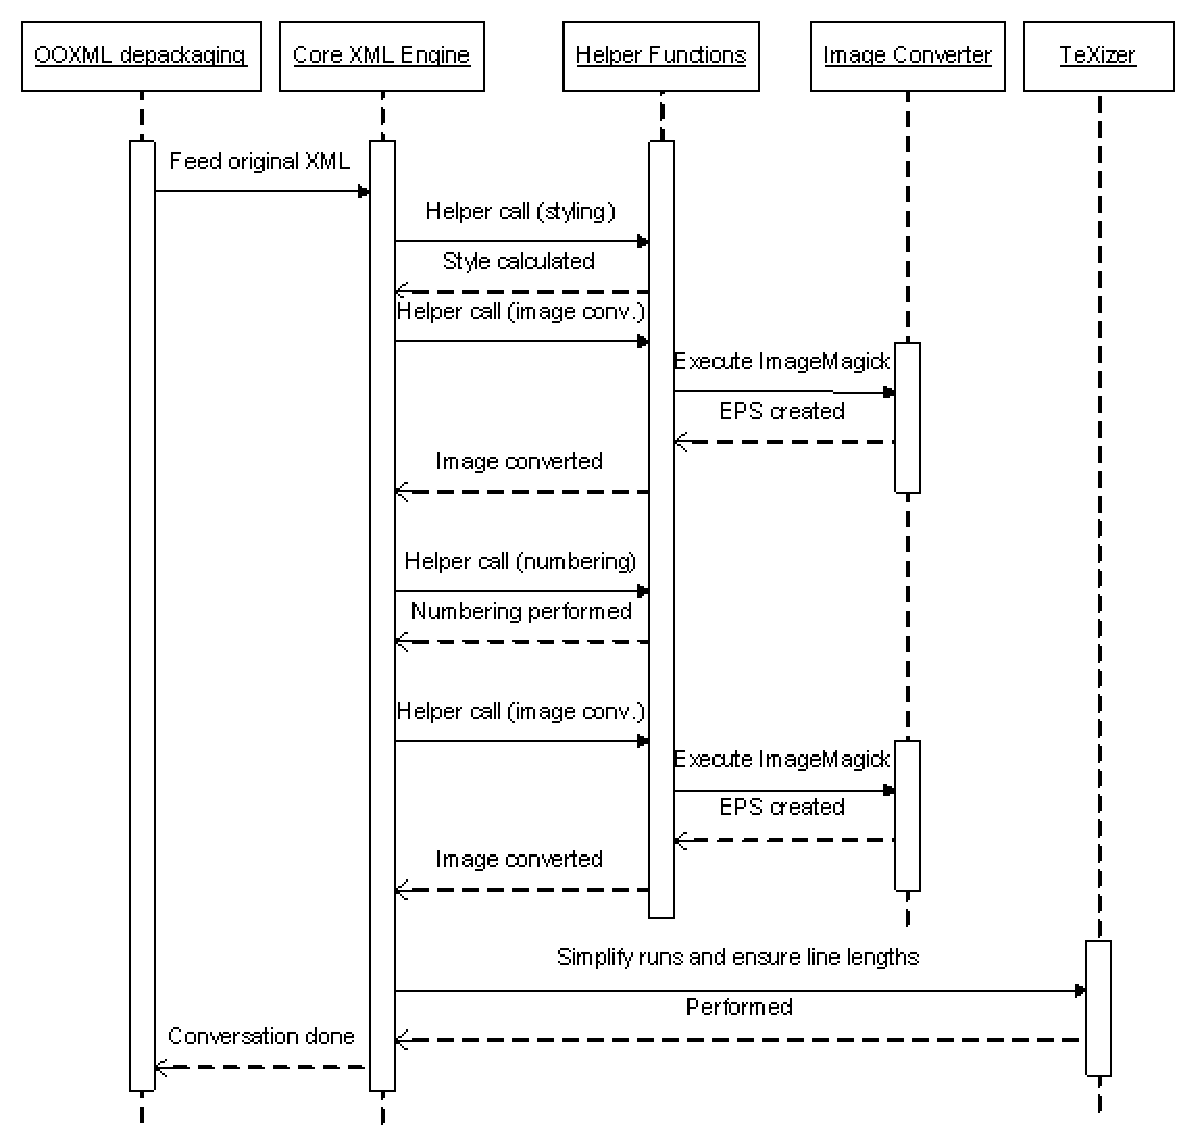
\includegraphics[width=10.52cm,height=8.41cm]{media/image1.eps}
\caption{\label{figure:_Ref186544261}: Figure caption}
\end{figure}
\end{verbatim}


The image is centered and the width and the height properties of the 
image are preserved. \textit{Image1.jpeg} was converted to \textit{
image1.eps} and the file was saved in the media subdirectory. When the 
image has a caption then it is also added to the output so that it can 
be referenced. 

Reference to the previous figure is described in OOXML in the following 
form:

\begin{verbatim}
<w:p w:rsidR="004F5706" w:rsidRPr="0030655B" w:rsidRDefault="004F5706" w:rsidP="004F5706">
  <w:pPr>
    <w:keepNext/>
  </w:pPr>
  <w:r w:rsidRPr="0030655B">
    <w:t xml:space="preserve">Reference to the figure: </w:t>
  </w:r>
  <w:r w:rsidR="007A289D">
    <w:fldChar w:fldCharType="begin"/>
  </w:r>
  <w:r w:rsidR="006B4DA8">
    <w:instrText xml:space="preserve"> REF _Ref186544261 \h </w:instrText>
  </w:r>
  <w:r w:rsidR="007A289D">
    <w:fldChar w:fldCharType="separate"/>
  </w:r>
  <w:r w:rsidR="006B4DA8">
    <w:t xml:space="preserve">Figure </w:t>
  </w:r>
  <w:r w:rsidR="006B4DA8">
    <w:rPr>
      <w:noProof/>
    </w:rPr>
    <w:t>1</w:t>
  </w:r>
  <w:r w:rsidR="007A289D">
    <w:fldChar w:fldCharType="end"/>
  </w:r>
</w:p>
\end{verbatim}


The generated TeX code is simple (it can be seen that the \textit{
Figure 1} text has been omitted from the output because it is internal 
to Word): 

\begin{verbatim}
Reference to the figure: \ref{figure:_Ref186544261}.
\end{verbatim}


Referencing tables is the same as for figures and sections, therefore we 
omit the referencing tables example.

\subsection{Lists and Tables}
There are two main categories of lists supported by OOXML and Word 2007:

\newcounter{numberedCntF}
\begin{enumerate}
\item Numbered and
\item Bulleted
\setcounter{numberedCntF}{\theenumi}
\end{enumerate}
Both numbered and bulleted lists are allowed to have multiple levels, 
while numbered lists can be continuous, which means that the list can be 
intermitted by some other content and then continued.

The first item of a numbered list looks the following:

\begin{verbatim}
<w:p w:rsidR="004F5706" w:rsidRPr="0030655B" w:rsidRDefault="004F5706" w:rsidP="004F5706">
  <w:pPr>
    <w:pStyle w:val="ListParagraph"/>
    <w:keepNext/>
    <w:numPr>
      <w:ilvl w:val="0"/>
      <w:numId w:val="1"/>
    </w:numPr>
  </w:pPr>
  <w:r w:rsidRPr="0030655B">
    <w:t>First</w:t>
  </w:r>
</w:p>
\end{verbatim}


The nodes embedded into \textit{$<$w:numPr$>$} and \textit{
$<$/w:numPr$>$} nodes specify that we have a list. The \textit{w:val} 
attributes of \textit{w:numId} and \textit{w:ilvl} specify numbering 
identifier and level parameters (style 1 at level 0 in our example). It 
may be abusing that the \textit{w:numPr} nodes describe both numbered 
and bulleted lists. It is the numbering identifier and the level 
parameter that distinguishes between the two categories of lists. These 
parameters are defined in \textit{numbering.xml} that is processed by 
docx2tex. The above element is the part of a complex multilevel numbered 
list:



\begin{verbatim}
\newcounter{numberedCntA}
\begin{enumerate}
\item First
\item Second
\item Third
\begin{enumerate}
\item First
\item Second
\item Third
\end{enumerate}
\item Fourth
\setcounter{numberedCntA}{\theenumi}
\end{enumerate}
\end{verbatim}


When a pervious list continues the 
$\backslash$setcounter\{enumi\}\{$\backslash$thenumberedCntA\} is 
inserted by docx2tex after the certain $\backslash$begin\{enumerate\}.

We omit showing a bulleted example since it differs only in the TeX 
output: uses the \textit{itemize} keyword instead of \textit{
enumerate} and do not have to maintain counters for continuous lists.



Docx2tex supports only simple tables therefore no merged, divided or 
differently aligned table cells are supported but the current features 
makes docx2tex to able to convert most of the tables.

There is no space to show the OOXML version of a simple table that has 
four cells. The generated TeX output is the following:



\begin{verbatim}
\begin{tabular}{|l|l|}
\hline
1 & 2 \\
\hline
3 & 4 \\
\hline
\end{tabular}
\caption{\label{table:_Ref186545972}: caption}
\end{table}
\end{verbatim}


\subsection{Special Characters}
TeX uses some special characters to place formatting commands to 
structure or change the appearance of text. When we want to place these 
special characters in fluent text they have to be described in a special 
way.

Consider the following set of special characters: $<$$>$ as'q \ldots \# 
$\backslash$ \{ \} \% \~ \_ \^{} \& \$ "\," \\
These are described in OOXML in the following form:

\begin{verbatim}
<w:p w:rsidR="00AB630B" w:rsidRDefault="00AB630B" w:rsidP="00AB630B">
  <w:r>
    <w:t xml:space="preserve">&lt;&gt; </w:t>
  </w:r>
  <w:proofErr w:type="spellStart"/>
  <w:r>
    <w:t>as'q</w:t>
  </w:r>
  <w:proofErr w:type="spellEnd"/>
  <w:r>
    <w:t xml:space="preserve"> ...# \ { } </w:t>
  </w:r>
  <w:proofErr w:type="gramStart"/>
  <w:r>
    <w:t>%  ~</w:t>
  </w:r>
  <w:proofErr w:type="gramEnd"/>
  <w:r>
    <w:t xml:space="preserve"> _ ^ &amp; $ ""</w:t>
  </w:r>
</w:p>
\end{verbatim}


The resulting TeX code is: 

\begin{verbatim}
$<$$>$ as'q ...\# $\backslash$ \{ \} \% \~ \_ \^ \& \$ "\,"
\end{verbatim}


\section{A Use Case}
Suppose the following scenario: Two authors decide to write a scientific 
article about their research topic and submit it to a conference or to a 
journal. First they split the proposed article to sections and assign 
each section to one of the authors. They start to work independently 
using Word 2007. After both of the authors finishes they merge the 
resulting text to one single document. After that step the first author 
reads though the whole document and makes changes using the Track 
Changes function of Word. The second author accepts or rejects the 
changes of the first author and also makes his changes using the Track 
Changes function of Word. When the authors agree that the quality of the 
article is acceptable then they convert it to TeX using docx2tex and 
apply special formatting required by the recommendation of the 
conference or journal. Now the article can be submitted.

The previous workflow is illustrated in \ref{figure:_Ref196063639}..

\begin{figure}[h]
\centering
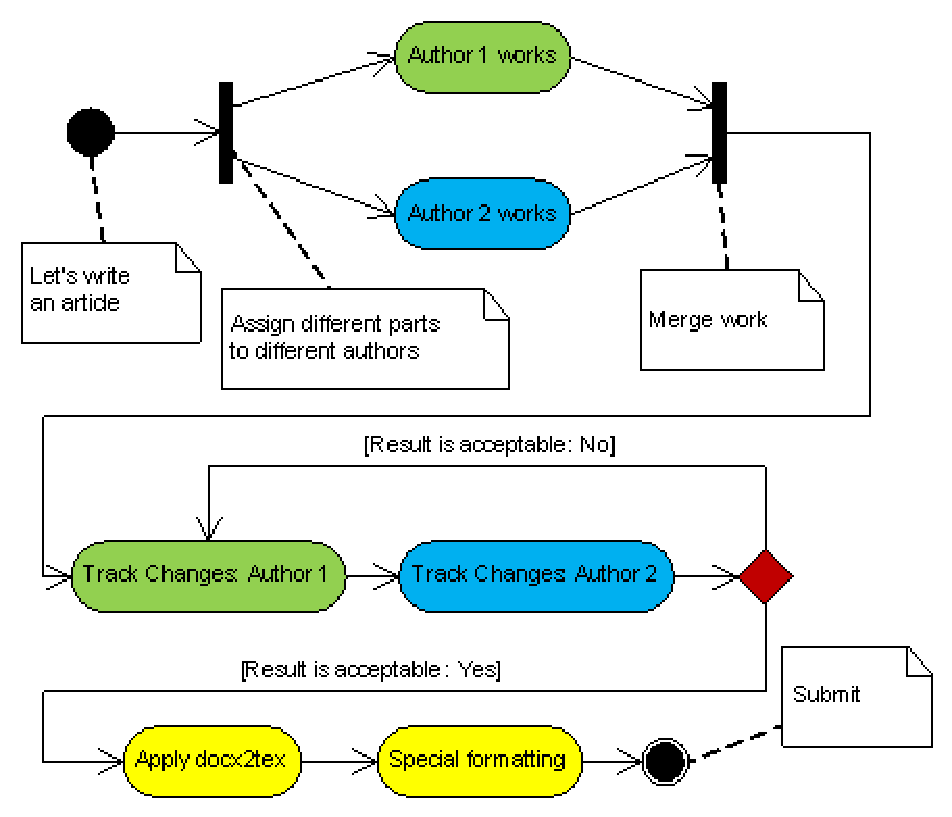
\includegraphics[width=12.55cm,height=10.68cm]{media/image2.eps}
\caption{\label{figure:_Ref196063639}: Workflow}
\end{figure}



As it can be seen we exploited the strengths of both the WYSIWYG Word 
2007 system to support effective team work and the typesetting TeX 
system to produce the best quality printout. The conversion between the 
file formats they use was performed using docx2tex. Note that docx2tex 
is able to do rough conversion and cannot apply special commands and 
styles.

Readers not familiar with the Track Changes function should consider 
\ref{figure:_Ref196063684}..\begin{figure}[h]
\centering
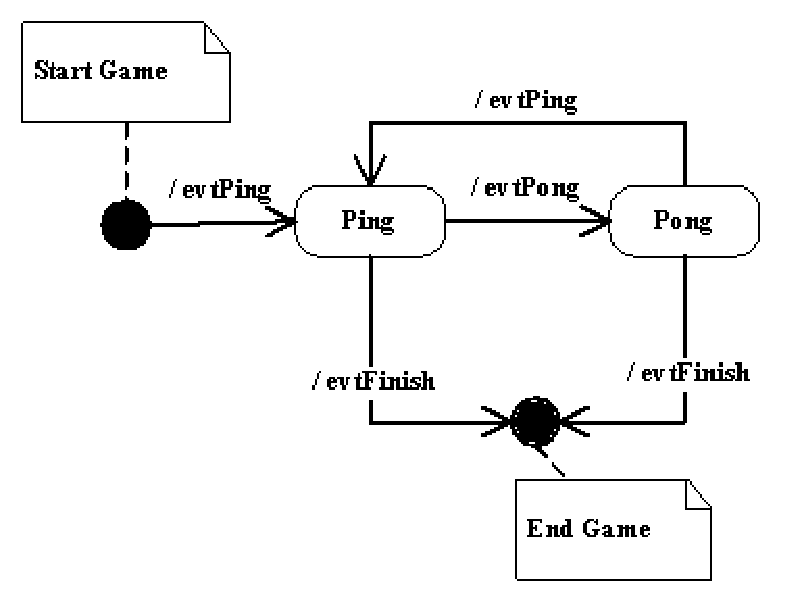
\includegraphics[width=15.17cm,height=12.60cm]{media/image3.eps}
\caption{\label{figure:_Ref196063684}: Track Changes function of Word}
\end{figure}



\section{Conclusion and Further Work}
In this article we introduced a tool called docx2tex that is dedicated 
to produce TeX documents from Word 2007 OOXML documents. The main 
advantage of this solution over classical methods is that we process the 
bare XML content of OOXML packages instead of processing binary files or 
exploiting the capabilities of the COM API of Word that makes our 
solution more robust and usable.

We presented the main features of docx2tex that are mostly related to 
text processing and formatting, structuring the document, handling 
images, tables and references. There are two important features that 
worth considering in the first place:

\newcounter{numberedCntE}
\begin{enumerate}
\item Equations
\item Embedded vector graphical drawings
\setcounter{numberedCntE}{\theenumi}
\end{enumerate}
Fortunately OOXML describes both of them in standard way therefore these 
contents can be converted to mathematical formulas of TeX and xfig 
respectively.

Multicolumn document handling and templating may also worth considering.

We plan to publish the application as a free and open source software 
therefore anybody can use it royalty free and add new features to the 
current feature set.

\section{References}
$[$1$]$ Article on What You See Is What You Get. 
http://en.wikipedia.org/wiki/WYSIWYG

$[$2$]$ Article on Microsoft Word. 
http://en.wikipedia.org/wiki/Microsoft\_Office\_Word

$[$3$]$ Product page of Microsoft Word. 
http://office.microsoft.com/en-us/word/FX100487981033.aspx

$[$4$]$ Article on TeX. http://en.wikipedia.org/wiki/TeX

$[$5$]$ Product page of Word2Tex. http://www.chikrii.com/

$[$6$]$ Product page of Word-to-LaTeX. 
http://kebrt.webz.cz/programs/word-to-latex/

$[$7$]$ Product page of OpenOffice.org. http://www.openoffice.org/

$[$8$]$ Project page of rtf2latex2e. 
http://sourceforge.net/projects/rtf2latex2e/

$[$9$]$ ECMA 376 OOXML Standard. 
http://www.ecma-international.org/publications/standards/Ecma-376.htm

$[$10$]$ ECMA 335 .NET CLI Standard. 
http://www.ecma-international.org/publications/standards/Ecma-335.htm

$[$11$]$ Link to ISO/IEC 23271:2006 Standard. 
http://standards.iso.org/ittf/PubliclyAvailableStandards/index.html

$[$12$]$ Project page of ImageMagick. http://www.imagemagick.org/



\end{document}
